%% fcup-thesis.tex -- document template for PhD theses at FCUP
%%
%% Copyright (c) 2015 João Faria <joao.faria@astro.up.pt>
%%
%% This work may be distributed and/or modified under the conditions of
%% the LaTeX Project Public License, either version 1.3c of this license
%% or (at your option) any later version.
%% The latest version of this license is in
%%     http://www.latex-project.org/lppl.txt
%% and version 1.3c or later is part of all distributions of LaTeX
%% version 2005/12/01 or later.
%%
%% This work has the LPPL maintenance status "maintained".
%%
%% The Current Maintainer of this work is
%% João Faria <joao.faria@astro.up.pt>.
%%
%% This work consists of the files listed in the accompanying README.

%% SUMMARY OF FEATURES:
%%
%% All environments, commands, and options provided by the `ut-thesis'
%% class will be described below, at the point where they should appear
%% in the document.  See the file `ut-thesis.cls' for more details.
%%
%% To explicitly set the pagestyle of any blank page inserted with
%% \cleardoublepage, use one of \clearemptydoublepage,
%% \clearplaindoublepage, \clearthesisdoublepage, or
%% \clearstandarddoublepage (to use the style currently in effect).
%%
%% For single-spaced quotes or quotations, use the `longquote' and
%% `longquotation' environments.


%%%%%%%%%%%%         PREAMBLE         %%%%%%%%%%%%

%%  - Default settings format a final copy (single-sided, normal
%%    margins, one-and-a-half-spaced with single-spaced notes).
%%  - For a rough copy (double-sided, normal margins, double-spaced,
%%    with the word "DRAFT" printed at each corner of every page), use
%%    the `draft' option.
%%  - The default global line spacing can be changed with one of the
%%    options `singlespaced', `onehalfspaced', or `doublespaced'.
%%  - Footnotes and marginal notes are all single-spaced by default, but
%%    can be made to have the same spacing as the rest of the document
%%    by using the option `standardspacednotes'.
%%  - The size of the margins can be changed with one of the options:
%%     . `narrowmargins' (1 1/4" left, 3/4" others),
%%     . `normalmargins' (1 1/4" left, 1" others),
%%     . `widemargins' (1 1/4" all),
%%     . `extrawidemargins' (1 1/2" all).
%%  - The pagestyle of "cleared" pages (empty pages inserted in
%%    two-sided documents to put the next page on the right-hand side)
%%    can be set with one of the options `cleardoublepagestyleempty',
%%    `cleardoublepagestyleplain', or `cleardoublepagestylestandard'.
%%  - Any other standard option for the `report' document arclass can be
%%    used to override the default or draft settings (such as `10pt',
%%    `11pt', `12pt'), and standard LaTeX packages can be used to
%%    further customize the layout and/or formatting of the document.

%% *** Add any desired options. ***
%PDF
%\documentclass[a4paper,narrowmargins,11pt,oneside,draft,onehalfspaced,singlespacednotes]{fcup-thesis}
%\documentclass[a4paper,narrowmargins,11pt,oneside,onehalfspaced,singlespacednotes]{fcup-thesis}
%Print
%\documentclass[draft,a4paper,narrowmargins,11pt,twoside,openright,onehalfspaced,singlespacednotes]{fcup-thesis}
\documentclass[a4paper,narrowmargins,11pt,twoside,openright,onehalfspaced,singlespacednotes]{fcup-thesis}

%% *** Add \usepackage declarations here. ***
%% The standard packages `geometry' and `setspace' are already loaded by
%% `ut-thesis' -- see their documentation for details of the features
%% they provide.  In particular, you may use the \geometry command here
%% to adjust the margins if none of the ut-thesis options are suitable
%% (see the `geometry' package for details).  You may also use the
%% \setstretch command to set the line spacing to a value other than
%% single, one-and-a-half, or double spaced (see the `setspace' package
%% for details).
% Overfull statements
\pretolerance=150
\setlength{\emergencystretch}{3em}
% Overfull end
\usepackage[english]{babel}
\usepackage{helvet} %To replace arial fonts
\usepackage{lipsum}
\usepackage[utf8]{inputenc}


%%% Additional useful packages
%%% ----------------------------------------------------------------
\usepackage{array}
\usepackage{amsmath}  
\usepackage{amssymb}
\usepackage{amsfonts}
\DeclareFontFamily{OT1}{pzc}{}
\DeclareFontShape{OT1}{pzc}{m}{it}{<-> s * [0.900] pzcmi7t}{}
\DeclareMathAlphabet{\mathpzc}{OT1}{pzc}{m}{it}
%Titles need to be 14 pt => Large in \normaltext 11pt
\usepackage{titlesec}
\titleformat*{\section}{\Large\bfseries}
\titleformat*{\subsection}{\Large\bfseries}
\titleformat*{\subsubsection}{\Large\bfseries}
%Titles need to be 14 pt => Large in \normaltext 11pt
\usepackage{amsthm}      
\usepackage[ruled,algochapter]{algorithm2e}
\usepackage{algorithmic}
\usepackage{bm}
\usepackage[mathscr]{euscript}
\usepackage{graphicx}       
\usepackage{psfrag}         
\usepackage{fancyvrb}    
\usepackage{float}
\usepackage{ltablex}
\usepackage[square,sort,comma,numbers]{natbib}        
\usepackage{bbding}         
\usepackage{dcolumn}        
\usepackage{booktabs} 
\usepackage{multirow}
\usepackage{paralist}     
\usepackage{ifdraft}  
\usepackage{indentfirst}    
\usepackage[nottoc,notlof,notlot]{tocbibind}
\usepackage{url}
\usepackage{tabularx}
%use font size for captions like 8pt -> normalisize 11pt, scriptsize->8pt
\usepackage[font={scriptsize}]{caption}
\usepackage[font={scriptsize}]{subcaption}
\captionsetup{font=scriptsize}

\usepackage[unicode]{hyperref}
\usepackage{xcolor}


\hypersetup{pdftitle=Obstacle avoidance framework based on reach sets, 
            pdfauthor=Alojz Gomola,
            colorlinks=false,
            urlcolor=blue,
            pdfstartview=FitH,
            pdfpagemode=UseOutlines,
            pdfnewwindow,
            breaklinks
          }
\usepackage{array}
\newcolumntype{L}[1]{>{\raggedright\let\newline\\\arraybackslash\hspace{0pt}}m{#1}}
\newcolumntype{C}[1]{>{\centering\let\newline\\\arraybackslash\hspace{0pt}}m{#1}}
\newcolumntype{R}[1]{>{\raggedleft\let\newline\\\arraybackslash\hspace{0pt}}m{#1}}         
\newcolumntype{B}{X}
\newcolumntype{S}[1]{>{\hsize=#1\textwidth}X}

\newcommand{\FIGDIR}{./Pics}    %%% directory containing figures
\newcommand{\twolinecellr}[2][r]{%
  \begin{tabular}[#1]{@{}r@{}}#2\end{tabular}}
\newcommand{\secState}[1]{
	\ifdraft{(#1) }{}
}
\theoremstyle{plain}
\newtheorem{theorem}{Theorem}
\newtheorem{lemma}[theorem]{Lemma}
\newtheorem{proposition}[theorem]{Proposition}

\theoremstyle{plain}
\newtheorem{definition}{Definition}
\newtheorem{problem}{Problem}
\newtheorem{example}{Example}
\newtheorem{assumption}{Assumption}

\theoremstyle{remark}
\newtheorem*{corollary}{Corollary}
\newtheorem*{note}{Note}




\newenvironment{dokaz}{
  \par\medskip\noindent
  \textit{Proof}.
}{
\newline
\rightline{\SquareCastShadowBottomRight}
}

\newenvironment{constraints}[1]{
  \par\medskip\noindent
  \textit{Constraints #1} \\
}{
\newline
\rightline{\SquareCastShadowBottomRight}
}


%\bibliographystyle{plainnat}     %% Author (year) style
\bibliographystyle{unsrt}        %% [number] style
\setcitestyle{square}

% Section  3.7 Challenge list
\newif\ifproblemchallenge   %# Build block for problem challenges
\problemchallengetrue       %# Show comments

\newcommand{\R}{\mathbb{R}}
\newcommand{\N}{\mathbb{N}}

\DeclareMathOperator{\pr}{\textsf{P}}
\DeclareMathOperator{\E}{\textsf{E}\,}
\DeclareMathOperator{\var}{\textrm{var}}
\DeclareMathOperator{\sd}{\textrm{sd}}


\newcommand{\T}[1]{#1^\top}        

\newcommand{\goto}{\rightarrow}
\newcommand{\gotop}{\stackrel{P}{\longrightarrow}}
\newcommand{\maon}[1]{o(n^{#1})}
\newcommand{\abs}[1]{\left|{#1}\right|}
\newcommand{\dint}{\int_0^\tau\!\!\int_0^\tau}
\newcommand{\isqr}[1]{\frac{1}{\sqrt{#1}}}
\newcommand{\norm}[1]{\left\lVert#1\right\rVert}


\newcommand{\pulrad}[1]{\raisebox{1.5ex}[0pt]{#1}}
\newcommand{\mc}[1]{\multicolumn{1}{c}{#1}}
\newcommand{\TBD}[1]{\color{red}\emph{--TBD:}#1\color{black}}

\usepackage{fontspec}
\setmainfont[
	Path={fonts/},
	UprightFont=*-Regular,
	ItalicFont=*-Italic,
	BoldFont=*-Bold,
	BoldItalicFont=*-Bold-Italic
]{Arial}

\newcommand{\hchapterspoce}{\hspace{20pt}}
\newcommand{\hsectuibspoce}{\hspace{15pt}}
\newcommand{\hsubsectuibspoce}{\hspace{10pt}}
\titleformat{\chapter}
	[hang]
	{\Huge}{Chapter \thechapter.\hchapterspoce}{0pt}{\Huge}[{\titlerule[1pt]}]
\titleformat{\section}[hang]{\huge}{\thesection.\hsectuibspoce}{0pt}{\huge}[{\titlerule[0.7pt]}]
\titleformat{\subsection}[hang]{\Large}{\thesubsection.\hsubsectuibspoce}{0pt}{\Large}[{\titlerule[0.4pt]}]

%%%%%%%%%%%%%%%%%%%%%%%%%%%%%%%%%%%%%%%%%%%%%%%%%%%%%%%%%%%%%%%%%%%%%%%%
%%                                                                    %%
%%                   ***   I M P O R T A N T   ***                    %%
%%                                                                    %%
%%  Fill in the following fields with the required information:       %%
%%   - \degree{...}       name of the degree obtained                 %%
%%   - \department{...}   name of the graduate department             %%
%%   - \gradyear{...}     year of graduation                          %%
%%   - \author{...}       name of the author                          %%
%%   - \title{...}        title of the thesis                         %%
%%%%%%%%%%%%%%%%%%%%%%%%%%%%%%%%%%%%%%%%%%%%%%%%%%%%%%%%%%%%%%%%%%%%%%%%

%% *** Change this example to appropriate values. ***
\degree{Doctor of Philosophy}
\department{Departamento de Matem\'{a}tica}
\gradyear{2019}
\author{Alojz Gomola}
\title{Obstacle Avoidance Framework based on Reach Sets}

%% *** NOTE ***
%% Put here all other formatting commands that belong in the preamble.
%% In particular, you should put all of your \newcommand's,
%% \newenvironment's, \newtheorem's, etc. (in other words, all the
%% global definitions that you will need throughout your thesis) in a
%% separate file and use "\input{filename}" to input it here.


%% *** Adjust the following settings as desired. ***

%% List only down to subsections in the table of contents;
%% 0=chapter, 1=section, 2=subsection, 3=subsubsection, etc.
\setcounter{tocdepth}{3}

%% Make each page fill up the entire page.
\flushbottom


%%%%%%%%%%%%      MAIN  DOCUMENT      %%%%%%%%%%%%

\begin{document}
%%%%%%%%%%%%%%%%%%%%%%%%%%%%%%%%%%%%%%%%%%%%%%%%%%%%%%%%%%%%%%%%%%%%%%%%
%%  Put your Chapters here; the easiest way to do this is to keep     %%
%%  each chapter in a separate file and `\include' all the files.     %%
%%  Each chapter file should start with "\chapter{ChapterName}".      %%
%%  Note that using `\include' instead of `\input' will make each     %%
%%  chapter start on a new page, and allow you to format only parts   %%
%%  of your thesis at a time by using `\includeonly'.                 %%
%%%%%%%%%%%%%%%%%%%%%%%%%%%%%%%%%%%%%%%%%%%%%%%%%%%%%%%%%%%%%%%%%%%%%%%%

%% *** Include chapter files here. ***
%01-Introduction
    \cleardoublepage
\chapter{\secState{R/W}Introduction}\label{ch:introduction}

\noindent This works present an approach based on \emph{reach set approximation} to \emph{detect \& avoid} various sort of threats in \emph{controlled/non-controlled} airspace environment. 

The \emph{motivation} is summarized in (sec. \ref{s:motivation}). The work \emph{goals} are given in (sec. \ref{s:goals}). A \emph{thesis organization} with notes is summarized in (sec. \ref{s:Overview}). A notable contributions of work are listed in (sec. \ref{s:Contributions}). The listing of student publications/technical reports/open source contributions are given in (sec. \ref{sec:listOfPublications}).
    \section{\secState{R}Motivation}\label{s:motivation}
\noindent The commercial potential of \emph{Unmanned Autonomous Systems} (UAS) is significant  enough to initiate one of the most significant changes in \emph{aviation} history \cite{airbusUTM2018blueprint}. The current \emph{usage} of UAS is limited by \emph{strict regulations} \cite{icao4444,icaoAnnex2,icaoAnnex11}. The goal is to enable \emph{full integration} of UAS in \emph{European airspace} by end of the year 2035 \cite{eurocontrol2018rpasatm}.


\begin{figure}[H]
    \centering
    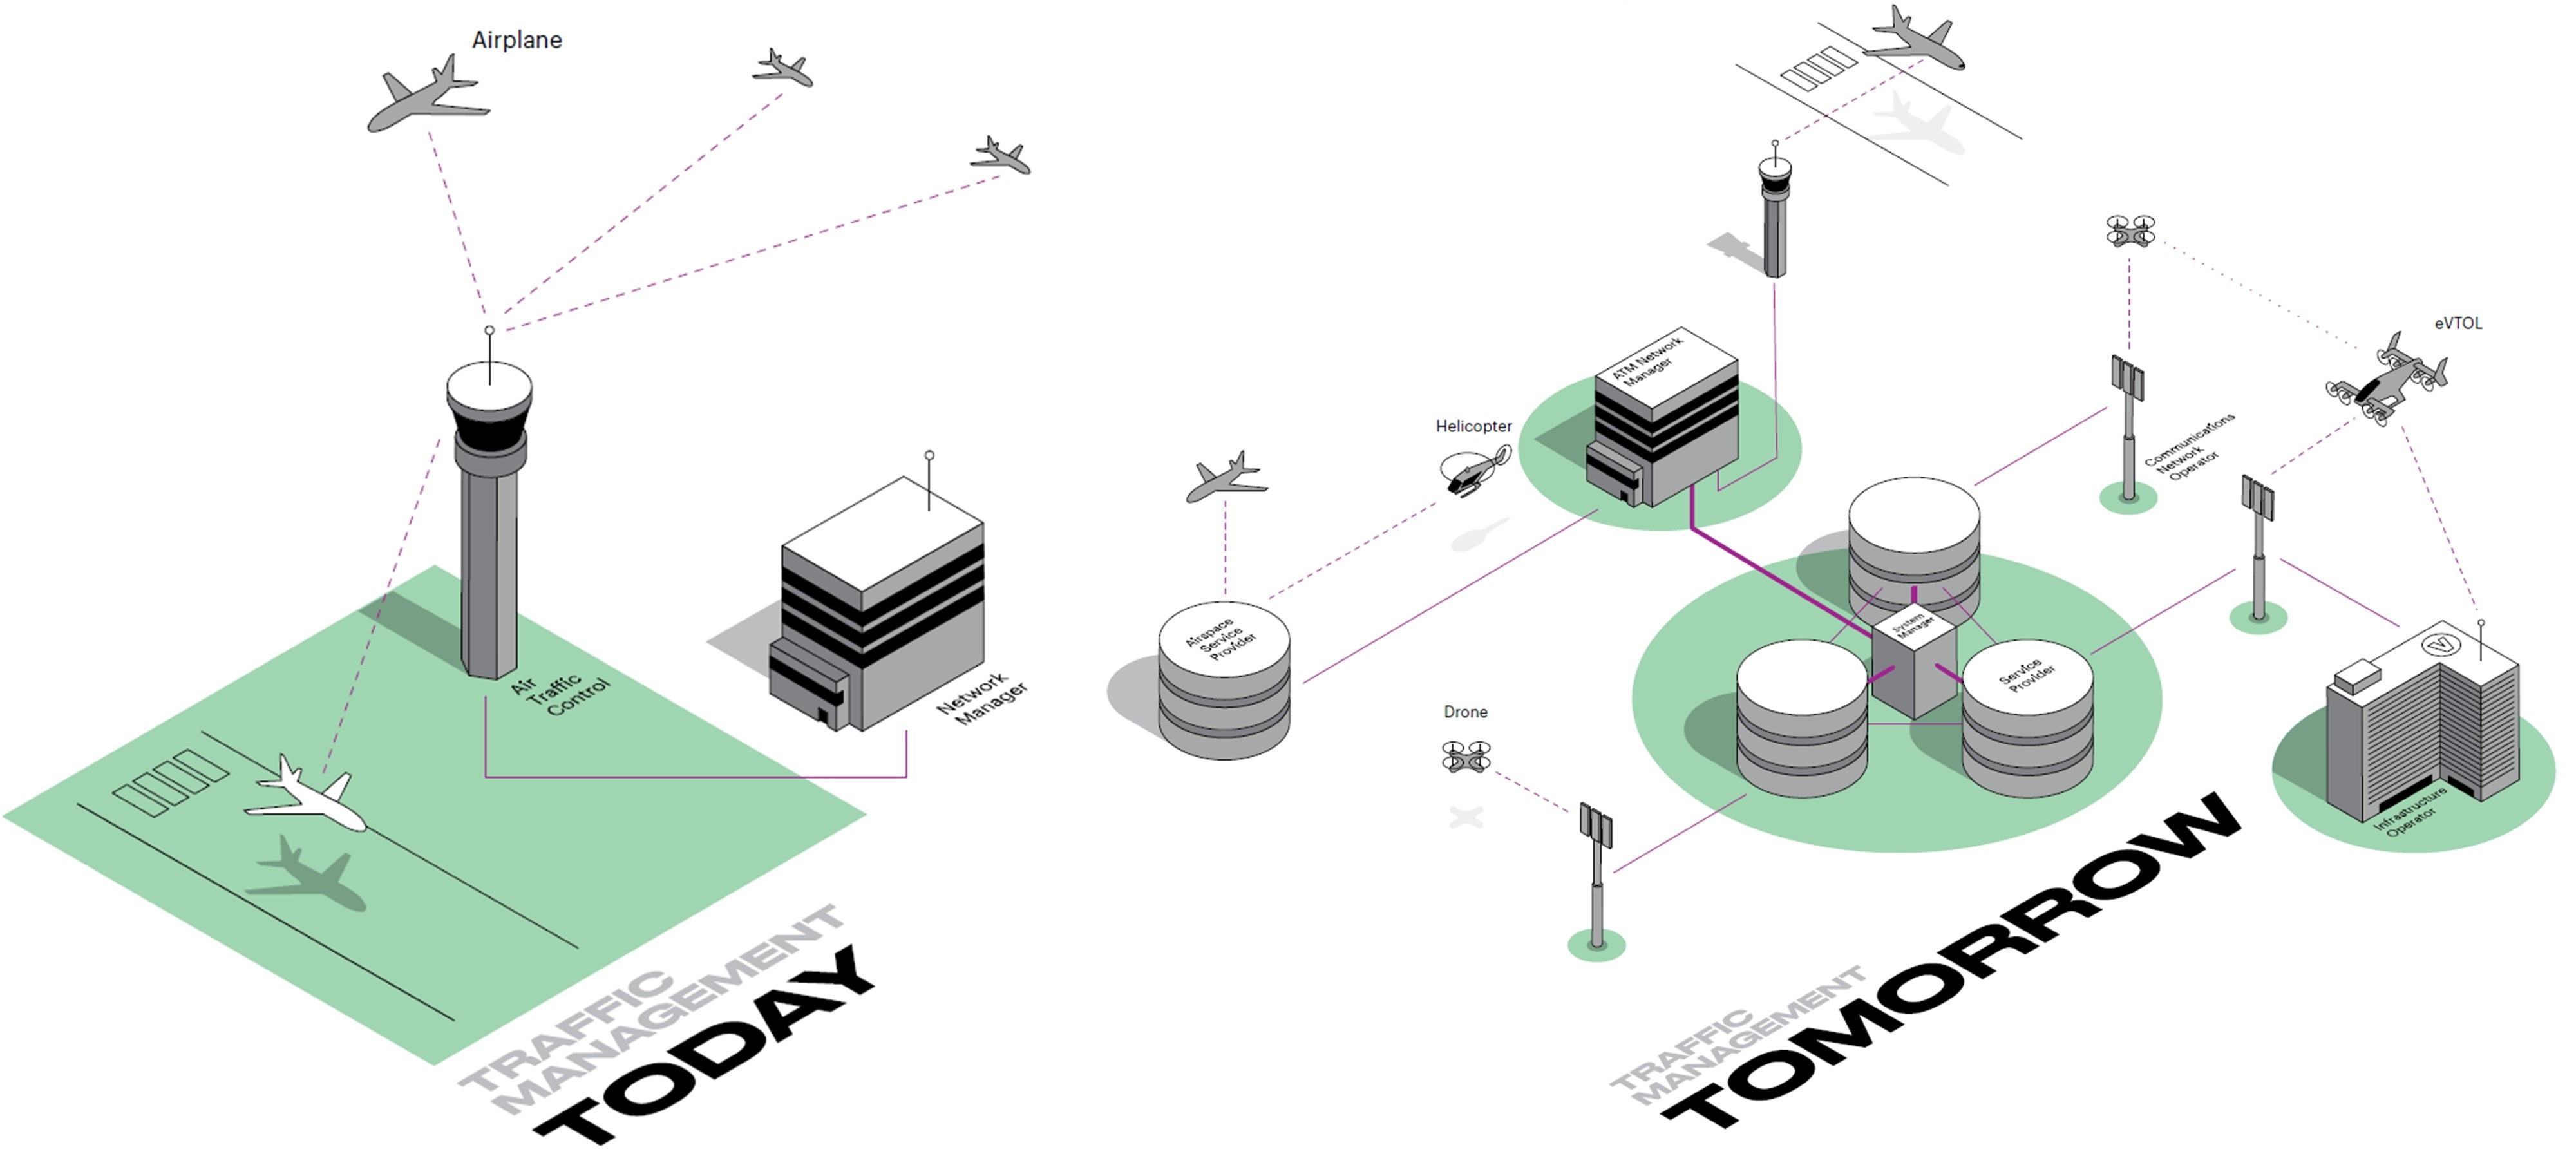
\includegraphics[width=0.9\textwidth]{\FIGDIR/I001TrafficManagement}
    \caption{Present and future \emph{Air Traffic Management} (ATC) \cite{airbusUTM2018blueprint}.}
    \label{fig:airTrafficManagementEvolution}
\end{figure}

\paragraph{UAS integraiton into Air Traffic:} The major effort is focused on \emph{Air Traffic Control} (ATC) changes. The \emph{actual} organization (sec. \ref{sec:AirspaceClassification}) and management (sec. \ref{sec:WellClear}) of airspace is centralized and \emph{human operated}.  

The \emph{ongoing changes} are shown in (fig. \ref{fig:airTrafficManagementEvolution}). The \emph{UAS Traffic Management} (UTM) (sec. \ref{sec:UTM}) complementing ATC is introduced to manage unmanned aviation. The additional traffic hubs, for UAS \emph{delivery \& transportation} services are added. The greatest change is on previously \emph{low-altitude uncontrolled} airspace, this space has new authority (UTM). The future UAS must implement mechanisms for \emph{event-based} navigation and avoidance (sec. \ref{sec:EventBasedAvoidance}).

Since 2014, there is a visible strong political support for developing rules on drones but regulations are harmonizing slowly. The European Aviation Safety Agency (EASA) has been tasked to develop a regulatory framework for drone operations and proposals for the regulation of "low-risk" UAV operations. In achieving this, EASA is working closely with the Joint Authorities for Regulation of Unmanned Systes (JARUS) \cite{jarus2016regulations}.

The \emph{operational rules} (sec. \ref{sec:AircraftOperationRules}) with \emph{rules of the air} \cite{icaoAnnex2} which are enforced now are simple. The \emph{future flight rules} (fig. \ref{fig:flightRulesIntro}) will be more complicated including the precise waypoint system and more complex missions. The future flight rules will be micro-managed by UTM. The example of such micro-management is shown in (sec. \ref{sec:UASTrafficManagement}, \ref{s:RuleEngineArchitecture}). 

The \emph{increase} of \emph{traffic density} increases the \emph{accident probability/severity}.  There are different threats endangering UAS, the \emph{obstacles} imposes eminent destruction threat, intruders can cooperate in mutual avoidance, the weather avoidance becomes more critical, the international/national authority can impose additional operational constraints. These threats needs to be well managed and prioritized to guarantee safe UAS operations.

\begin{figure}[H]
    \centering
    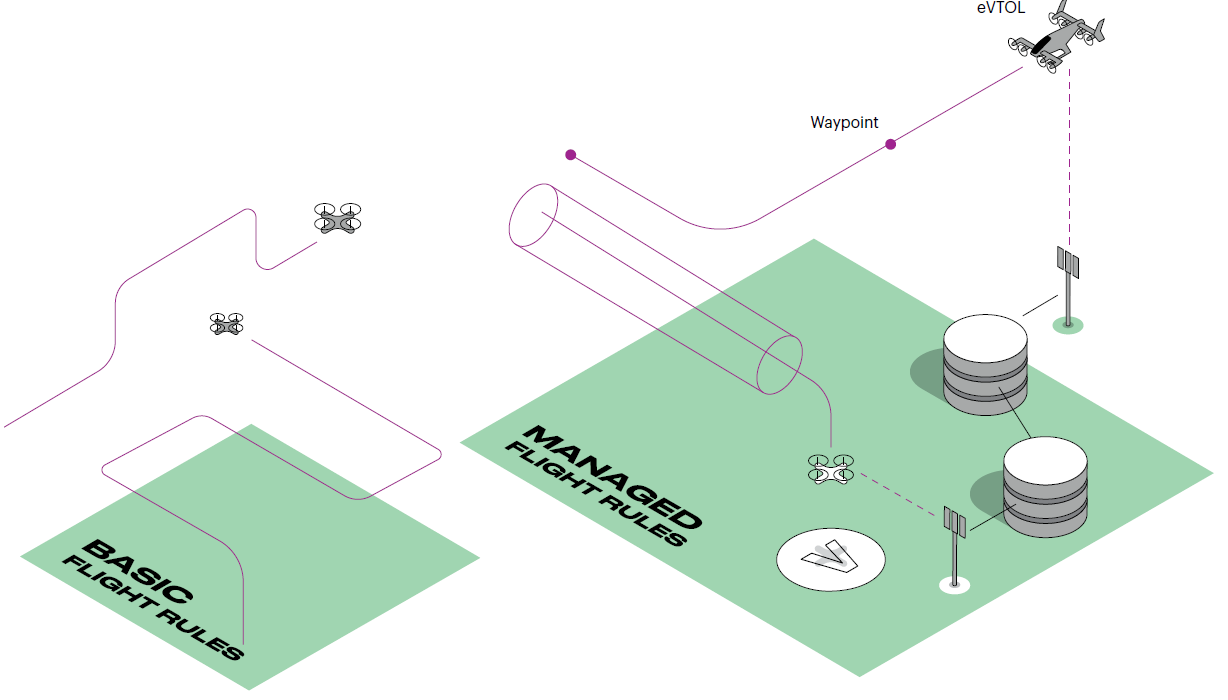
\includegraphics[width=0.8\textwidth]{\FIGDIR/I002FlightRules}
    \caption{Flight rules overview. \cite{airbusUTM2018blueprint}.}
    \label{fig:flightRulesIntro}
\end{figure}

\paragraph{Detect \& Avoid:} The other approach is bottom-up, that means the development of basic adaptable functionality to cover complex navigation/avoidance tasks in \emph{controlled airspace}. The intuitive definition of \emph{Detect \& Avoid} (DAA) functionality is given in (fig. \ref{fig:detectAdnAvoidIntroduction}).

\begin{figure}[H]
    \centering
    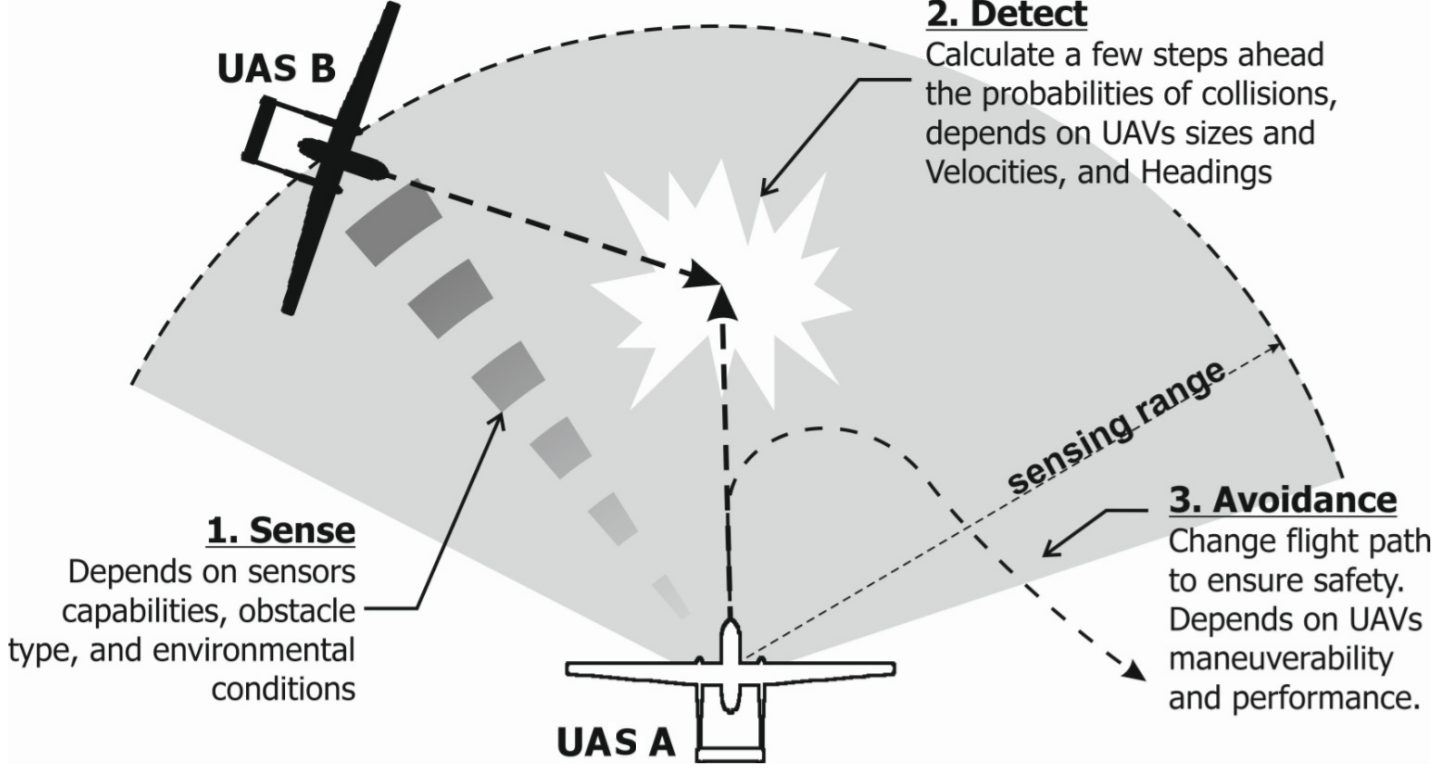
\includegraphics[width=0.6\textwidth]{\FIGDIR/I003DetectAndAvoid}
    \caption{\emph{Detect \& Avoid} (DAA) principle \cite{jenie2014velocity}.}
    \label{fig:detectAdnAvoidIntroduction}
\end{figure}

\noindent The DAA can be applied in short term (avoidance) and long term (navigation) tasks. It consist from three continuously repeating major steps:
\begin{enumerate}
    \item \emph{Sense} - the processing of intermediate sensor reading, the physical world approximation creation.
    
    \item \emph{Detect} - an addition of information from other sources to create complex situation assessment scenario, future possibilities projection and control strategy selection.
    
    \item \emph{Avoid} - execution of selected control strategy while checking possible changing events.
\end{enumerate}

The \emph{short term avoidance} (sec. \ref{s:aviudabceGridRun}) can be chained into \emph{long term navigation} (sec. \ref{s:missionControlRun}). This long term navigation can be used to solve \emph{UTM/ATM} imposed constraints, under assumption that there is sufficient \emph{data fusion} (sec. \ref{s:sensorFusion}).

\paragraph{Challenge Motivation:} Both \emph{Air Traffic Control} and \emph{Detect \& Avoid} requires a tool to assess possible UAS maneuvering:

\begin{enumerate}
    \item \emph{Air Traffic Control} needs to know the UAS maneuvering capabilities in order to \emph{validate} feasibility of \emph{issued orders} and to predict future \emph{trajectory} for \emph{collision prevention}.
    
    \item \emph{Detect \& Avoid} needs to calculate feasible \emph{system constraints feasible maneuvering strategy} in finite time to ensure own safety. 
\end{enumerate}

\paragraph{Reach Sets:} These challenges are addressable by employment of \emph{reach sets} (sec. \ref{s:ReachSets}). The \emph{reach set} is self-validating set of possible maneuvering strategies for some initial UAS state and some time-period. 

To guarantee finite time evaluation, the discretization of \emph{operation space} (sec. \ref{s:AvoidanceGrid}) and \emph{movement discretization} (sec. \ref{sec:MovementAutomatonBackground}) needs to be introduced. The discretization gives finite countable sets of choices, therefore it also guarantees finite time evaluation process.

Our \emph{implementation} of \emph{reach set approximation} (sec. \ref{s:reachSet}) enables to encode some sought behavioral patterns as natural properties (sec. \ref{s:constrainedTrajectoryExpansion}). This enables to generate specific task oriented \emph{reach set approximation} for navigation (sec. \ref{s:chaoticReachSet}), avoidance (sec. \ref{s:harmonicReachSet}), UTM behavior predictions (sec. \ref{sec:collisionCase}). 


    \section{Goals}\label{s:goals}
\paragraph{Situation:} The \emph{UAS} equipped with cooperative/non-cooperative surveillance sensors, with prior knowledge of operation space has to fly a mission represented ordered set of waypoints. The set of sensors can change depending on UAS construction. The minimal airworthiness for a given operation is assumed.

\paragraph{Problem:} Given environment and artifact definitions (sec. \ref{s:basicDefinitions}) with \emph{initial assumptions} (sec. \ref{s:initialAssumptions}) and \emph{incremental problem definition} (sec. \ref{s:IncrementalProblemDefinition}) develop \emph{obstacle avoidance framework} which will satisfy \emph{avoidance} (sec. \ref{s:AvoidanceRequirements}) and \emph{navigation} (sec. \ref{s:navigationRequirements}).

\paragraph{Expected Solution:} Define an approach based on \emph{reach sets} which are capable of:

\begin{enumerate}
    \item \emph{Static obstacle avoidance} - to avoid the ground, man-made structures in open terrain. 
    
    \item \emph{Intruders avoidance} - to avoid flying objects which does not have the intention to harm our UAS, detected in sufficient distance. 

    \item \emph{Geo-fencing support} - to avoid known zones/airspace portions, which have forbidden entry.

    \item \emph{Weather avoidance} - to avoid known zones of harmful weather conditions.

    \item \emph{Cooperative conflict resolution} - to communicate own position to authority and to follow authority orders.
    
    \item \emph{Treat prioritization} - to assess avoidance according to natural or man-made priorities. (Rather break geo-fence, than crashing into the ground).
\end{enumerate}

\paragraph{Validation:} Develop test-framework to showcase approach properties. Define \emph{test scenarios} (sec. \ref{s:testingApproach}) to validate \emph{Expected Solution Performance} (sec.  tab. \ref{tab:testCasesSummary}) concerning \emph{avoidance capability} (sec. \ref{s:performanceEvaluationTable}) and \emph{computational feasibility} (sec. \ref{s:ComputaitonFootprint}).

\paragraph{Application Requirements:} There are  following application requirements, based on similar applications for \emph{manned aviation} and \emph{industry expectations}:

\begin{enumerate}
    \item \emph{Low-performance requirements} - the computational footprint of the approach should be polynomial. The most of actual UAS systems have \emph{embedded computer} with low computation power.
    
    \item \emph{Deterministic} - the \emph{avoidance strategy} should be achieved in finite time frame. The mandatory requirement for \emph{airborne operation support application}, the advice needs to be reproducible under the same conditions.
    
    \item \emph{Scalability} - the \emph{avoidance framework} should be portable to the different platforms, and it should work with different sensor array. The interface requirement for \emph{control} and \emph{data fusion} coming from other \emph{collision avoidance systems}.
    
    \item \emph{Adaptability} - the \emph{avoidance process} should have tuning points where is possible to change behavior according to UAS context. The regulations are changing with location, time and circumstances, the part of calculation/control process needs to be implemented dynamically.
\end{enumerate}
    \section{ Overview}\label{s:Overview}

\noindent The thesis is organized like follows:

\begin{enumerate}
    \item \emph{Introduction} (ch. \ref{ch:introduction}) - the introduction chapter giving an overview of work motivation, goals, contributions and \emph{author`s list of publication}.
    
    \item \emph{Collision Avoidance} (ch. \ref{ch:CollisionAvoidance}) - This chapter gives aerospace-related background. The manned aviation is serving as the knowledge base for an assumption of future UAS Detect \& Avoid functionality. The chapter gives overview of airspace classification, which told us where and what we can do or expect. Aircraft operational rules for general are reflected into \emph{separation functionality}. The separation can be passively enforced by Air Traffic Management authority or active enforced by \emph{ACAS-X/TCAS} systems. The \emph{UAS Traffic Management} is parallel to manned aviation practices with additional layer of complexity.  The \emph{Event-Based avoidance} is introduced to give overview of concepts used later.
    
    \item \emph{Background Theory} (ch. \ref{ch:backGroundTheory}) - this chapter outlines background necessary for approach understanding. The \emph{control theory} system models are used as a base for the \emph{reach set} calculation. The important concept of \emph{hybrid automaton} (special case of hybrid automaton) is introduced. The LiDAR related theory and complements are presented at last. 
    
    \item \emph{Problem Statement} (ch. \ref{c:problemStatement}) - this chapter states the problem solved in this work. The basic definition and terminology are established at beginning with initial problem and assumptions. Incremental problem is introduced with increasing complexity and relaxed conditions. Avoidance and Navigation functional and non-functional requirements are stated at last. 
    
    \item \emph{State of Art} (ch. \ref{ch:stateOfArt}) - this chapter covers important results of other researcher works in topics of Movement Automaton, Sensor \& Data Fusion, Navigation Algorithm, Reach Sets, and Testing Approach. The \emph{UAS Traffic Management} concept relevant to this work is introduced.  
    
    \item \emph{Approach} (ch. \ref{ch:approach}) - this chapter describes the approach, it starts with an overview (sec. \ref{s:approachOverview}), outlining the block scheme of the system (fig. \ref{fig:AvoidanceFrameworkConceptNew}). The discretization of the space, trajectories, and system model are covered in (sec. \ref{s:modelMAImplementation} - \ref{s:AvoidanceGrid}), the following topics are covered:
    \begin{enumerate}[a.]
        \item \emph{Reach Set Estimation} (sec. \ref{s:reachSet}) - the discretization, performance evaluation, and generation algorithms.
        
        \item \emph{Encounter Modeling} (sec. \ref{s:staticObstacles} - \ref{s:intruders}) - static obstacles, intruders, static/moving constraints, and more.
        
        \item \emph{Collision Avoidance} (sec. \ref{s:avoidanceConcept}) - the avoidance/navigation loop with global data fusion procedure, complexity and safety margin calculations.
        
        \item \emph{Further to Cooperative Operations} (sec. \ref{sec:UASTrafficManagement} - \ref{sec:ruleEngine}) - the approach to satisfy scalability and \emph{UTM} requirements.
    \end{enumerate}
    
    \item \emph{Simulations} (ch. \ref{Simulations}) the simulations cover aspects developed in approach, the test plan (tab. \ref{tab:testCasesSummary}) summarizes test cases. The results are outlined in (tab. \ref{tab:testCasesPerformacneEvaluation}), the computation load statistics are summarized in (tab. \ref{tab:computationLoadStatistics}). The tests are divided into the following categories:
    
    \begin{enumerate}[a.]
        \item \emph{Non-cooperative Test Cases} (sec. \ref{s:noncooperativeTestCases}) - various obstacles, weather constraints, and non-cooperative intruders test cases
    
        \item \emph{Cooperative Test Cases} (sec. \ref{s:cooperativeTestCases}) - maneuvers in controlled airspace under supervision of traffic management.
    
        \item \emph{Reach Set Estimation Performance and Properties} (sec. \ref{sec:reducedReachSetPerformance}) - the comparison of various estimation methods, the impact on complexity.
    \end{enumerate}
    
    \item \emph{Conclusion and Future Work} (ch. \ref{ch:Conclusion}) - work conclusion, summarizing achieved results, comparing other approaches, outlining reusable modular parts of approach, utilizing the future work on approach shortcomings.
\end{enumerate}
    \section{(R) Contributions}\label{s:Contributions} 
\noindent The \emph{contributions} of this work can be divined into two categories:
    
\paragraph{Conceptual Contributions:} The contributions enhancing and enriching the conceptual level of \emph{Detect \& Avoid} systems, namely:

\begin{enumerate}
    \item \emph{Movement automaton control and prediction} -  necessity to abstract the control of the system from the \emph{detect and avoid} systems, leads to customization of hybrid automaton (sec. \ref{s:HybridAutomaton}) to \emph{movement automaton} (def. \ref{s:MovementAutomatonDefinitionAndProperties}). The movement automaton can be adapted to nonlinear system (sec. \ref{s:UASNonlinearModel}) as a instance (sec. \ref{s:movementAutomatonDefinition}). The movement automaton can be also used as a predictor of the system (sec. \ref{s:referenceTrajectoryGenerator}). The \emph{initial state disparity issue} \cite{gomola2017obstacle} has been addressed in (sec. \ref{s:segmentedMovementAutomaton}).
    
    \item \emph{Trajectory as a discrete command chain} -  the \emph{movement automaton} as a control interface consuming the discrete command chain enabled the \emph{finite discrete representation} of trajectory (eq. \ref{eq:ourTrajectoryImplementation}).
    
    \item \emph{Reach set discretization} - the \emph{infinite reach set} (def. \ref{}) can be represented as a tree of movements from system initial state (def. \ref{def:ReachSetApproximationByMovementAutomaton}). This tree can have associated properties, like reachibility of each trajectory segment (eq. \ref{eq:trajectoryReachibility}).  The advantage of having finite maneuver set, with little precision sacrifice, which can be calculated prior the flight have huge impact on \emph{computation complexity} (sec. \ref{sec:MCRcomputationalComplexity}). Enabling to use approach on different platforms with small computational power. 
    
    \item \emph{Operational space assessment} - the operational space is separated by grid into finite set of the cells. Each cell has properties to track like the occurrence of obstacle, presence of intruder or impact of constraint. The \emph universal data fusion procedure (sec. \ref{s:sensorFusion}) is enabling accumulation of treat information from various sources.
    
    \item \emph{Hierarchical threat assessment} -  the \emph{various threat} sources (obstacles, intruders, constraints) are categorized according to operational environment/rules and their avoidance priority is handled according to that (fig. \ref{fig:missionControlRunActivityDiagram}).
    
    \item \emph{UAS Traffic Management} - the architecture proposal for traffic management  as cooperative authority (sec. \ref{sec:utmArchitecture}) covers some basic maneuvers (sec. \ref{sec:handlingHeadOnApproach}, \ref{sec:handlingConvergingManuever},\ref{sec:handlingOvertakeManuever}), the more important is the adaptability of presented approach to cooperative (sec. \ref{sec:cooperativeConflictResolution}) and non-cooperative (sec. \ref{sec:nonCooperativeConflictResolution}) avoidance modes, showing adaptability. 
\end{enumerate}

\paragraph{Implementation Contributions:} The concepts, which solve implementation issues for \emph{Detect \& Avoid} systems, namely:

\begin{enumerate}
    \item \emph{Operational space segmentation} - the \emph{planar grid} (sec. \ref{s:AvoidanceGrid}) slice (fig. \ref{fig:LidarSpaceSegmentation}) have been selected, because it can be used for fast assessment of LiDAR scan data to estimate, obstacle (\ref{fig:P01CountOfLiDARHits}) or visibility (\ref{fig:P02OvershadowedMapobstacle}). The cell volume is increasing with distance from UAS, this gives us decreased space status assessment complexity.
    
    \item \emph{Wave-front algorithm for avoidance estimation} - to estimate reach set the space exploration method has been developed. The \emph{rapid exploration tree} (fig. \ref{fig:rapidExplorationTrajectoryTree}) is employed as \emph{wave-front} expansion (alg. \ref{alg:Wavefront Propagation}). Various shapes and properties of \emph{reach set estimation} can be achieved employing the \emph{constrained expansion functions} for \emph{chaotic} (alg. \ref{alg:ExpansionConstraintFunctionForChaoticReachSet}), harmonic (alg. \ref{alg:ExpansionConstraintFunctionForHarmonicReachSet}), and, \emph{ACAS-like} (alg. \ref{alg:ExpansionConstraintFunctionForACASLikeReachSet}) reach set approximations.
    
    \item \emph{Encounter and constraints models} - the planar grid used in solution required a development of encounter models for static obstacles, constraints (sec. \ref{s:staticObstacles}), intruders, moving constraints (sec. \ref{s:intruders}). The intersection algorithms can be reused in other approaches using unusual grid.
    
    \item \emph{Avoidance process enhancement (Rule engine)} - the air traffic rules are changing based on time and geographic location, the UTM concept is under development. These reasons are calling to use flexible implementation architecture, rule engine (sec. \ref{s:RuleEngineArchitecture}). The rule engine can be set to cover any kind of rules (fig. \ref{fig:RuleEngineInstanceLevels}).
\end{enumerate}
    \section{\secState{R}List of Publications}\label{sec:listOfPublications}

\noindent This \emph{section} contains the list of published articles, proceedings, technical reports and module projects, relevant to the \emph{thesis topic}.

%   My First Article Ever!
\paragraph{Article:} Alojz Gomola, Joao Borges de Sousa, Fernando Lobo Pereira, and Pavel Klang. Obstacle avoidance framework based on reach sets. In Iberian Robotics conference, pages 768–779. Springer, 2017. \cite{gomola2017obstacle}\footnote{Draft available online: \url{https://goo.gl/kZujZE}}.

\emph{Summary:} This report on preliminary investigations concerning the development of a LiDAR-based detect and avoid (DAA) system with a low computational footprint for small Unmanned Air Systems. The focus is on the integration with nominal flight control systems and computational feasibility. The proposed system decomposes the SAA problem into the following components detection, space assessment, escape trajectory estimation and avoidance execution. The control logic is encoded with the help of a hybrid automaton. The properties of the system are studied with the help of approximations to time slices of the UAV reach set.


\paragraph{Article:}  Juraj {\v{S}}tevek,  Michal  Kvasnica,  Miroslav  Fikar,  and  Alojz  Gomola. A  parametric programming  approach  to  automated  integrated  circuit  design. IEEE Transactions on Control Systems Technology, 26(4):1180–1191, 2018. \cite{vstevek2018parametric}\footnote{IEEE copy online: \url{https://ieeexplore.ieee.org/stamp/stamp.jsp?arnumber=7981386}}.

\emph{Summary:} The proposal of an optimization-based slotting approach to automated \emph{integrated circuit} design for generating a power transistor. The original slotting problem is formulated as a mixed-integer linear program. It is solved through parametric optimization with an advantage that usage of any commercial optimization solvers on user’s side is avoided with short evaluation time and simple implementation. The approach is applied in specific very large scale integration production technology and demonstrated on an example.

\emph{Contributions:} Point-location algorithm for MPC region selection. 

\paragraph{Proceedings:} Kristian Klausen, Jostein Borgen Moe, Jonathan Cornel van den Hoorn, Alojz Gomola, Thor I Fossen, and Tor Arne Johansen. Coordinated control concept for recovery of a fixed-wing uav on a ship using a net carried by multirotor UAVs.  In Unmanned Aircraft Systems (ICUAS), 2016 International Conference on, pages 964–973. IEEE, 2016, \cite{klausen2016coordinated}\footnote{Public copy available online: \url{http://folk.ntnu.no/torarnj/ICUAS2016_singlecolumn.pdf}}.

\emph{Summary:} Ship-based Unmanned Aerial Vehicle (UAV) operations represent an important field of research which enables a large variety of mission types. Most of these operations demand a high level of endurance which normally requires the use of a fixed-wing UAV. Traditionally, a net located on the ship deck is used for recovering the fixed-wing UAV. However, there are numerous challenges when attempting autonomous landings in such environments. Waves will induce heave motion, and turbulence near the ship will make approaches challenging. In this paper, we present a concept using multi-rotor UAVs to move the recovery operation off the ship deck. To recover the fixed-wing UAV, a net is suspended below two coordinated multirotor UAVs which can synchronize the movement with the fixed-wing UAV. The approach trajectory can be optimized with respect to the wind direction, and turbulence caused by the ship can be avoided. In addition, the multirotor UAVs can transport the net at a certain speed along the trajectory of the fixed-wing UAV, thus decreasing the relative velocity between the net and fixed-wing UAV to reduce the forces of impact. This paper proves the proposed concept through a simulation study and a preliminary control system architecture.

\emph{Contributions:} Ground station maneuver implementation, messaging between ground station/UAVs. RTK-GPS for precise navigation integration, Net-release mechanism design, Mechanical parts for 3D printer modeling. 

\paragraph{Proceedings:}  Alojz Gomola.  An aspect-oriented solution for mutual exclusion in embedded systems. In Alena Kozakova, editor, ELITECH15: 17th Conference of doctoral students, pages 964–973, Bratislava, Slovak Republic, May 2015. Online publication, \cite{gomola2015aspectOriented}\footnote{Draft available online: \url{https://github.com/logomo/Elitech15-paper}}.

\emph{Summary:} Embedded systems are developed for a wide range of applications. The best-known applications are industrial process control and banking solutions. Fault tolerance is a crucial requirement in long-term embedded systems. This paper presents solution for mutual exclusion in embedded systems. The usual mutual exclusion solution using semaphores is a crosscutting concern. Semaphores are difficult to maintain in code, and their failure rate is high. We propose new aspect-oriented solution for mutual exclusion. Our solution utilizes aspect-oriented approach, is usable in other systems and designed to be robust against program changes, and it provides a solution to aspect fragility problem.

\paragraph{Technical report:} Alojz Gomola, Pavel Klang, and Jan Ludvik. Probabilistic approach in data fusion for obstacle avoidance framework based on reach sets. In Internal publication collection, pages 1–93. Honeywell, 2017, \cite{gomola2017probabilistic}\footnote{Public copy available online: \url{https://github.com/logomo/Data-Fusion-Report}}.

\emph{Summary:} The \emph{sensor input} and \emph{information sources} fusion procedure design to obtain rated space assessment for visibility, obstacle occupancy, and reachability evaluation. A unique statistical approach was proposed to couple partial ratings under reading and time uncertainty. The key contribution is scalable approach to evaluate \emph{UAS action space} and \emph{Feasible Trajectories} properties. 

\paragraph{Technical report:}  Alojz Gomola. Model predictive control of unmanned air vehicles with obstacle avoidance capabilities, technical report, FEUP, 2017, \cite{gomola2017mpc}\footnote{Public copy available online: \url{https://github.com/logomo/Predictive-control---Final-report}}.

\emph{Summary:} Initial solution of \emph{predictive control} problem for \emph{UAS} navigation in constrained, non-controlled airspace. The key contribution is \emph{Movement Automaton} (a special type of hybrid automaton) establishment in current form (sec. \ref{sec:MovementAutomatonBackground}). The \emph{stability}, \emph{controllability} and \emph{observability} properties have been proven. The \emph{feasibility} of \emph{Movement Automaton} as \emph{control interface} and \emph{future state predictor} has been shown through formal proof and excessive testing.

\paragraph{Technical report:} Alojz  Gomola.   Optimal  control  of  unmanned  air  vehicles  with  obstacle  avoidance capabilities in partially known environment.  Technical report, FEUP, 2017. \cite{gomola2017optimal}\footnote{Public copy available online: \url{https://github.com/logomo/Optimal-Control}}.

\emph{Summary:} The \emph{optimization problem} for \emph{obstacle avoidance} (eq. \ref{eq:trajectoryTrackingOptimalizaitonProblem}) to satisfy \emph{avoidance requirements} (sec. \ref{s:AvoidanceRequirements}) 

\paragraph{Framework:} Feature-based ACAS\footnote{Matlab prototype available online: \url{https://github.com/logomo/Feature-based-ACAS}} implementation to support claims of this work has been developed through the course of years \emph{2016-2019}. The framework provides: 
\begin{enumerate}
    \item \emph{Simulation environment} - full support for single/multiple UAS simulation support in controlled/non-controlled airspace.
    
    \item \emph{Mission Control Support} - standard mission control support for \emph{sparse ordered waypoint} mission type. 
    
    \item \emph{UAS Traffic Management} - support for \emph{collaborative} weather and collision avoidance with general authority in controlled airspace. The configurable \emph{event-handling} through \emph{rule-engine}.
    
    \item \emph{Encounter Models} - the model for \emph{static obstacles} supporting point-cloud generation of LiDAR sensor, various intruders model supporting the ADS-B like encounter model, static/dynamic polygon constraints with altitude range. 
    
    \item \emph{Collision Avoidance} - the support for \emph{cooperative} and \emph{non-cooperative} behavior in controlled airspace, \emph{non-collaborative, non-adversary} behavior in non-controlled airspace. 
    
    \item \emph{Reach Set Estimation Methods} - four methods for various property focused \emph{Reach Set Estimations}.
\end{enumerate}


	
%% This adds a line for the Bibliography in the Table of Contents.
\addcontentsline{toc}{chapter}{Bibliography}
%% *** Set the bibliography style. ***
%% (change according to your preference/requirements)
%\bibliographystyle{plain}
%% *** Set the bibliography file. ***
%% ("thesis.bib" by default; change as needed)
\bibliography{thesis}

%% *** NOTE ***
%% If you don't use bibliography files, comment out the previous line
%% and use \begin{thebibliography}...\end{thebibliography}.  (In that
%% case, you should probably put the bibliography in a separate file and
%% `\include' or `\input' it here).

\end{document}
